% !TeX spellcheck = pt_PT
%
%
% Apêndice 1
%
\chapter{Apêndice A} \label{ap:exemplo}
O Apêndice A contem o diagrama de todas as entidades e as suas propriedades.

\begin{figure}[h]
	\begin{center}
		\resizebox{150mm}{!}{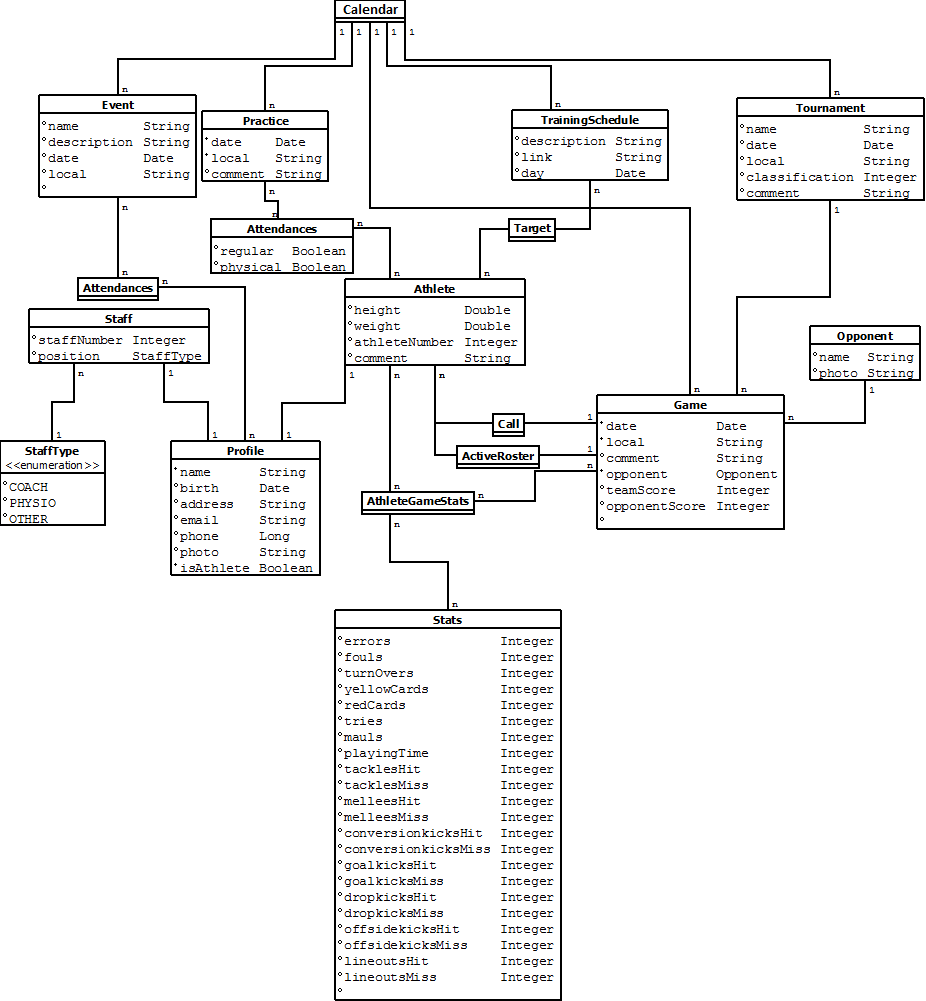
\includegraphics{./figures/diagram.png}}
	\end{center}
	\caption{Diagrama de Entidades}\label{fig:}
\end{figure}



A lista de entidades representa as propriedades que são tipos primitivos pelo seu nome(id,height,weight), as propriedades que referem associações de um para um pelo nome da entidade a que está associada(\emph{Profile}), e as propriedades que referem associações de um para muitos por uma lista de entidades a que está associada(List$<$\emph{Event}$>$).


Lista de Entidades
\begin{enumerate}
	\item \emph{Athlete}	(id,height,weight,athleteNumber,comment,\emph{Profile},List$<$\emph{Practice}$>$,List$<$\emph{TrainingSchedule}$>$,
	List$<$\emph{Game}$>$,List$<$\emph{AthleteGameStats}$>$)
	\item \emph{AthleteGameStats} (id,\emph{Athlete},\emph{Stats},\emph{Game})
	\item \emph{Event} (id,name,description,date,local,List$<$\emph{Profile}$>$)
	\item \emph{Game} (id,date,local,comment,\emph{Opponent},List$<$\emph{Athlete}$>$,List$<$\emph{AthleteGameStats}$>$)
	\item \emph{Opponent}
	(id,name,photo)
	\item \emph{Practice} (id,date,local,comment,List$<$\emph{Athlete}$>$)
	\item \emph{Profile} (id,name,birth,address,mail,phone,photo,List$<$\emph{Event}$>$)
	\item \emph{Staff} (id,staffNumber,\emph{Profile},\emph{StaffType})
	\item \emph{StaffType}(id,name)
	\item \emph{Stats} (id,errors,fouls,turnOvers,yellowCards,redCards,tries,mauls,playingTime,\emph{Tackle},\emph{Mellee},\\
	\emph{ConvertionKick},\emph{GoalKick},\emph{DropKick},\emph{OffSide},\emph{LineOut},List$<$\emph{AthleteGameStats}$>$)
	\item \emph{Tackle} (tackleHits,tackleMiss)
	\item \emph{Mellee} (melleeHits,melleeMiss)
	\item \emph{ConvertionKick} (convertionKickHits,convertionKickMiss)
	\item \emph{GoalKick} (goalkickHits,goalkickMiss)
	\item \emph{DropKick} (dropKickHits,dropkickMiss)
	\item \emph{OffSideKick} (offsideHits,offsideMiss)
	\item \emph{LineOut} (lineOutHits,lineOutMiss)
	\item \emph{Tournament} (id,classification,comment)
	\item \emph{TrainingSchedule} (id,description,link,date,List$<$\emph{Athlete}$>$)
\end{enumerate}
Todas estas entidades foram implementadas diretamente na camada do Modelo.
\newpage